% Лабораторная работа по криптографии № 3
% Михедов Константин Константинович

% Тип документа: статья, на бумаге А4
\documentclass[a4paper]{article}

% Подключение сторонних tex файлов 
\usepackage{import}


% Основные данные - ВУЗ, факультет, город...
\import{./../../stuff/tex}{config.tex}
% Небольшой набор инструментов
\import{./../../stuff/tex}{tools.tex}

% Подключение необходимых зависимостей
\import{./../../stuff/tex/settings}{packages.tex}
% Настройка подключенных пакетов
\import{./../../stuff/tex/settings}{preferences.tex}


% Шаблон титульной страницы 
\import{./../../stuff/tex/templates}{title.tex}
% Упрощенный блок "выполнил"
\import{./../../stuff/tex/templates}{sign2.tex}
% Макрос для содержания
\import{./../../stuff/tex/templates}{toc.tex}

% Определяем название документа
\title{
  ОТЧЕТ \\
  О ПРАКТИЧЕСКОЙ РАБОТЕ №3 \\
  по дисциплине <<Основы криптографии и стеганографии>> \\
  ШИФРЫ ГАММИРОВАНИЯ
}
% Указываем преподавателя
\renewcommand{\teachername}{
    Заведующий кафедрой информационной безопасности киберфизических систем \\
    канд. техн. наук, доцент \\
    \entryline{3.5cm} О.О. Евсютин
}


% Путь до внешних изображений
\graphicspath{ {./figures/}}
% Нумеруем все формулы
\mathtoolsset{showonlyrefs=false}


% Основной текст работы
\begin{document}
  \templatedtitlepage
  
  \toc

  \section{Здание на практическую работу}

  Целью данной практической работы является программная реализация и последующий 
  криптоанализ некоторых блочных шифров.

  В рамках работы необходимо выполнить следующие шаги:

  \begin{enumerate}
    \setlength{\itemindent}{1cm}
    \item {
        Программно реализовать шифр Виженера с несколькими способами выработки
        гаммы на основе серкретного ключа шифрования:

        \begin{itemize}
            \setlength{\itemindent}{1cm}
            \item Повторение короткого лозунга
            \item Самоключ по открытому тексту
            \item Самоключ по закрытому тексту
        \end{itemize}
    }
    \item {
        Изучить и описать методы криптографического анализа данного шифра и его модификаций 
    }
    \item {
        Провести криптоанализ данных шифров
    }
    \item {
        Подготовить отчет о проделанной работе
    }
  \end{enumerate}

  \newpage
  \section{Краткая теоретическая часть}

  \subsection{Описание шифра Виженера}

  Пусть дан исходный алфавит $A$ мощности $m$, каждый элемент которого
  можно представить элементом множества $\mathbb{Z}_m = \left\{x, x \in \mathbb{Z} \text{ и } 0 \leq x < m \right\}$.
  Тогда если задан открытый текст $X = \left\{x_1, x_2, \dots x_n\right\}$ и некий ключ
  для формирования гаммы $K_r = \left\{k_1, k_2, \dots, k_r\right\}$, то сначала
  по какому-то правилу вырабатывается гамма - $\Gamma = \left\{\gamma_1, \gamma_2, \dots, \gamma_n\right\}$, при помощи которой
  уже и происходит получение зашифрованного сообщения $Y = \left\{y_1, y_2, \dots, y_n\right\}$:
  \begin{equation}
    y_i = (x_i + \gamma_i) \mod m
  \end{equation}

  Для расшифровки требуется каким-то образом получить используемую для шифрования гамму,
  после чего исходное сообщение вычисляется очень просто:
  \begin{equation}
    x_i = (y_i - \gamma_i) \mod m
  \end{equation}

  В данном криптографическом алгоритме очень многое, в частности его устойчивость к криптоанализу,
  зависит от способа выработки гаммы и метода ее получения для расшифровки.

  \subsection{Методы выработки гаммы}

  \subsubsection{Повторение короткого лозунга}

  Для данного метода требуется ключ произвольной длины $r$: $K_r = \left\{k_1, k_2,  \dots, k_r\right\}$,
  после чего символы гаммы рекуррентно вычисляются по следующей формуле:
  \begin{equation}
    \gamma_i = k_{\left(i\mod{r}\right)}
  \end{equation}

  Гамму необходимо выработать такой же длины, как и исходное сообщение для зашифрования или расшифрования.
  При расшифровании необходимо знать весь ключ, тогда по нему снова будет выработанна вся гамма.

  \subsubsection{Самоключ по открытому тексту}

  Для данного метода выработки гаммы требуется ключ длиной в один символ, то есть по факту $k$,
  тогда вся гамма определяется этим ключом и символами открытого текста:
  \begin{equation}
    \Gamma = \left\{k, x_1, x_2, \dots, x_{n - 1}\right\}
  \end{equation}

  При расшифровке сообщения при помощи ключа вычисляется первый символ исходного сообщение,
  благодаря которому расшифровывается второй и так далее (гамма при расшифровке вырабатывается постепенно).

  \subsubsection{Самоключ по закрытому тексту}

  Для данного метода выработки гаммы требуется ключ длиной в один символ -  $k$,
  затем с его помощью вычисляется первый симв шифртекста, который становиться вторым
  символом гаммы:
  \begin{equation}
    \Gamma = \left\{k, y_1, y_2, \dots, y_{n - 1}\right\}
  \end{equation}

  То есть выработка гаммы в процессе зашифрования происходит постепенно (в противовес
  выработке по открытому тексту).

  \subsection{Методы криптоанализа Шифра Виженера}

  Стоит отметить, что сообщения, зашифрованные с гаммой, выработанной по шифртексту,
  очень легко расшифровать, так как вся гамма по факту в открытом виде содержится
  в шифртексте. Да, для того, чтобы узнать первый символ исходного сообщение, все таки
  придется подобрать ключ, но так как этот ключ состоит всего из одного символа,
  то его подбор даже в алфавите огромной мощности не займет много времени.

  \subsubsection{Метод грубой силы}

  При использовании повторяющегося короткого лозунка в качестве гаммы подобрать ключ
  может быть довольно сложно. Во-первых, злоумышленнику неизвестна длина ключа, поэтому
  ему придется перебрать все возможные ключи всех возможных длин, что при достаточно мощном
  алфавите займет достаточно времени.

  При иных способах выработки гаммы все гораздо проще - необходимо просто перебрать все символы
  алфавита, что вычислительно не очень сложно даже при использовании \textit{Unicode}.

  \subsubsection{Применение частотного анализа}

  Не смотря на то, что шифр Виженера гораздо меньше подвержен частотному анализу, нежели например
  шифр Цезаря, с некотороми доработками его можно применить (рационально только при гамме,
  выработанно с помощью повторения короткого лозунга).

  \paragraph{Определение длины ключа}

  Чтобы было возможным использовать частотный анализ, необходимо разбить шифртекста на
  группы символов, сдвиг которых ($\gamma_i$) одинаков, для чего и требуется знание длины ключа.
  Так как он повторяется - сделать такое разбиение очень просто.

  Чтобы определить длину ключа (предположительно), необходимо воспользоваться
  тем, что ключ неоднократно повторяется, а в языке много часто встречающихся повторяющийхся последовательностей
  (например в английском языке можно часто заметить последовательность \textit{th}).

  Посчитаем количество одинаковых символов для шифртекста и шифртекста сдвинутого вправо на
  какое-то количество символов:
  \begin{table}[H]
    \centering
    \begin{tabular}{| c | r | c |}
      \hline
      Сдвиг & Шифртекст & Совпадения \\
      \hline
      0 & VVHQWVVRMHUSGJG  & - (15) \\
      \hline
      1 &  vVHQWvVRMHUSGJ  & 2 \\ 
      \hline
      2 &   VVHQWVVRMHUSg  & 1 \\ 
      \hline
      3 &    VVHQWVVRMHUS  & 0 \\ 
      \hline
      4 &     VvHQWVVRMHU  & 1 \\ 
      \hline
      5 &      vvHQWVVRMH  & 2 \\ 
      \hline
      6 &       vVHQWVVRM  & 1 \\ 
      \hline
      7 &        VVHQWVVR  & 0 \\ 
      \hline
      8 &         VVHQWVV  & 0 \\ 
      \hline
      9 &          VVHQWV  & 0 \\ 
      \hline
      10 &           VVHQW & 0 \\ 
      \hline
      11 &            VVHQ & 0 \\ 
      \hline
      12 &             VVH & 0 \\ 
      \hline
      13 &              VV & 0 \\ 
      \hline
      14 &               V & 0 \\ 
      \hline
    \end{tabular}
  \end{table}

  Можно заметить одинаковое количество совпадений на различных значениях сдвига,
  в частности например при сдвигах в 1 и 5, и при сдвигах в 2 и 6. Разница между
  значенимяи сдвига в обоих случаях равняется 4, что позволяет предположить, что длина
  ключа в наиболее вероятном случае равна 4.

  \paragraph{Разделение на группы символов}

  Далее весь шифртекст необходимо разделить на группы символов, которые находятся друг
  от дрга на расстоянии длины ключа, то есть:
  \begin{equation}
    \textit{abcdef} \overset{r = 3}{\longrightarrow} \left\{\left\{a,d\right\}, \left\{b,e\right\}, \left\{c,f\right\}\right\}
  \end{equation}

  \paragraph{Непосредственно частотный анализ}

  Каждую из полученных групп символов подвергают частотному анализу. Так как значение сдвига
  каждого символа в группе одинаково (ключ повторяется), то все символы в группе действительно
  подвержены стандартной частотности языка.
  Благодаря частотному анализу вычисляется сдвиг для каждой группы (по аналогии с тем,
  как это делается для шифра Цезаря), после чего на основе этих значений собирается полный ключ.

  \newpage
  \section{Примеры ручного шифрования}

  В процессе зашифрования и расшифрования используется английский алфавит, состоящий из
  галавных букв (мощность такого алфавита равна 26).

  \subsection{Гамма - повторение коротного лозунга}

  Выполним зашифрование слова \textbf{YANDEX} при помощи ключа \textbf{CAT}.
  Для начала представим ключ в численном виде:
  \begin{eqnarray}
    CAT = \left\{2, 0, 19\right\}
  \end{eqnarray}

  Далее выработаем гамму необходимой длины при помощи повторения:
  \begin{equation}
    \Gamma = \left\{2, 0, 19, 2, 0, 19\right\}
  \end{equation}

  Теперь представить открытый текст в символьном виде и выполним зашифрование:
  \begin{equation}
    \begin{aligned}
      Y = 24 \rightarrow (24 + 2) &\mod 26 = 0 \rightarrow A \\
      A = 0 \rightarrow (0 + 0) &\mod 26 = 0 \rightarrow A \\
      N = 13 \rightarrow (13 + 19) &\mod 26 = 6 \rightarrow G \\
      D = 3 \rightarrow (3 + 2) &\mod 26 = 5 \rightarrow F \\
      E = 4 \rightarrow (4 + 0) &\mod 26 = 4 \rightarrow E \\
      X = 23 \rightarrow (23 + 19) &\mod 26 = 16 \rightarrow Q \\
    \end{aligned}
  \end{equation}

  Получается необходимый шифртекст - \textbf{AAGFEQ}, выполним расшифрование:
  \begin{equation}
    \begin{aligned}
      A = 0 \rightarrow (0 - 2) &\mod 26 = 24 \rightarrow Y \\
      A = 0 \rightarrow (0 - 0) &\mod 26 = 0 \rightarrow A \\
      G = 6 \rightarrow (6 - 19) &\mod 26 = 13 \rightarrow N \\
      F = 5 \rightarrow (5 - 2) &\mod 26 = 3 \rightarrow D \\
      E = 4 \rightarrow (4 - 0) &\mod 26 = 4 \rightarrow E \\
      Q = 16 \rightarrow (16 - 19) &\mod 26 = 23 \rightarrow X \\
    \end{aligned}
  \end{equation}

  Расшифрование выполнено успешно.

  \subsection{Гамма - выработка по открытому тексту}

  Зашифруем слово \textbf{MONEY} при помощи ключа \textbf{K} ($= 10$).
  Представим откртый текст в численном виде:
  \begin{equation}
    MONEY = \left\{12, 14, 13, 4, 24\right\}
  \end{equation}

  Составим гамму на основе открытого текста и ключа:
  \begin{equation}
    \Gamma = \left\{ 10, 12, 14, 13, 4\right\}
  \end{equation}

  Выполним зашифрование:
  \begin{equation}
    \begin{aligned}
      M = 12 \rightarrow (12 + 10) &\mod 26 = 22 \rightarrow W \\ 
      O = 14 \rightarrow (14 + 12) &\mod 26 = 0 \rightarrow A \\ 
      N = 13 \rightarrow (13 + 14) &\mod 26 = 1 \rightarrow B \\ 
      E = 4 \rightarrow (4 + 13) &\mod 26 = 17 \rightarrow R \\ 
      Y = 24 \rightarrow (24 + 4) &\mod 26 = 2 \rightarrow C \\ 
    \end{aligned}
  \end{equation}

  В результате зашифрования получен шифртекст \textbf{WABRC}, расшифруем его, зная только ключ.

  Получим первый символ открытого текста:
  \begin{equation}
    W = 22 \rightarrow (22 - 10) \mod 26 = 12 \rightarrow M
  \end{equation}

  Теперь, когда мы знаем первый символ открытого текста, можно расшифровать и второй:
  \begin{equation}
    A = 0 \rightarrow (0 - 12) \mod 26 = 14 \rightarrow O
  \end{equation}

  Аналогичным образом вычисляются все последующие символы - из кода предыдущих:
  \begin{equation}
    \begin{aligned}
      B = 1 \rightarrow (1 - 14) &\mod 26 = 13 \rightarrow N \\ 
      R = 17 \rightarrow (17 - 13) &\mod 26 = 4 \rightarrow E \\ 
      C = 2 \rightarrow (2 - 4) &\mod 26 = 24 \rightarrow Y \\ 
    \end{aligned}
  \end{equation}

  Расшифрование выполнено успешно.

  \subsection{Гамма - выработка по закрытому тексту}

  Зашифруем слово \textbf{BANG} при помощи ключа \textbf{F} ($ = 5$). Для начала представим
  открытый текст в численном виде:
  \begin{equation}
    BANG = \left\{1, 0, 13, 6\right\}
  \end{equation}

  Теперь зашифруем первый символ при помощи ключа:
  \begin{equation}
    B = 1 \rightarrow (1 + 5) \mod 26 = 6 \rightarrow G
  \end{equation}

  Исходя из первого символа шифртекста и второго открытого, получим второй:
  \begin{equation}
    A = 0 \rightarrow (0 + 6) \mod 26 = 6 \rightarrow G
  \end{equation}

  Исходя из второго символа шифртекста и третьего открытого, получим тертий:
  \begin{equation}
    N = 13 \rightarrow (13 + 6) \mod 26 = 19 \rightarrow T
  \end{equation}

  И наконец, из третьего символа шифртектса и четвертого открытого, получим последний символ шифртекста:
  \begin{equation}
    G = 6 \rightarrow (6 + 19) \mod 26 = 25 \rightarrow Z
  \end{equation}

  В ходе зашифрования был получен шифртекст \textbf{GGTZ}, расшифруем его.
  Зная ключ и шифртекст можно получить всю необходимую для расшифрования гамму:
  \begin{equation}
    \Gamma = \left\{ 5, 6, 6, 19 \right\}
  \end{equation}

  Выполним расшифрование с ее помощью:
  \begin{equation}
    \begin{aligned}  
      G = 6 \rightarrow (6 - 5) &\mod 26 = 1 \rightarrow B \\ 
      G = 6 \rightarrow (6 - 6) &\mod 26 = 0 \rightarrow A \\ 
      T = 19 \rightarrow (19 - 6) &\mod 26 = 13 \rightarrow N \\ 
      Z = 25 \rightarrow (25 - 19) &\mod 26 = 6 \rightarrow G \\  
    \end{aligned}
  \end{equation}

  Расшифрование выполнено успешно.

  \newpage
  \section{Демонстрация работы программы}

  \begin{figure}[H]
    \centering
    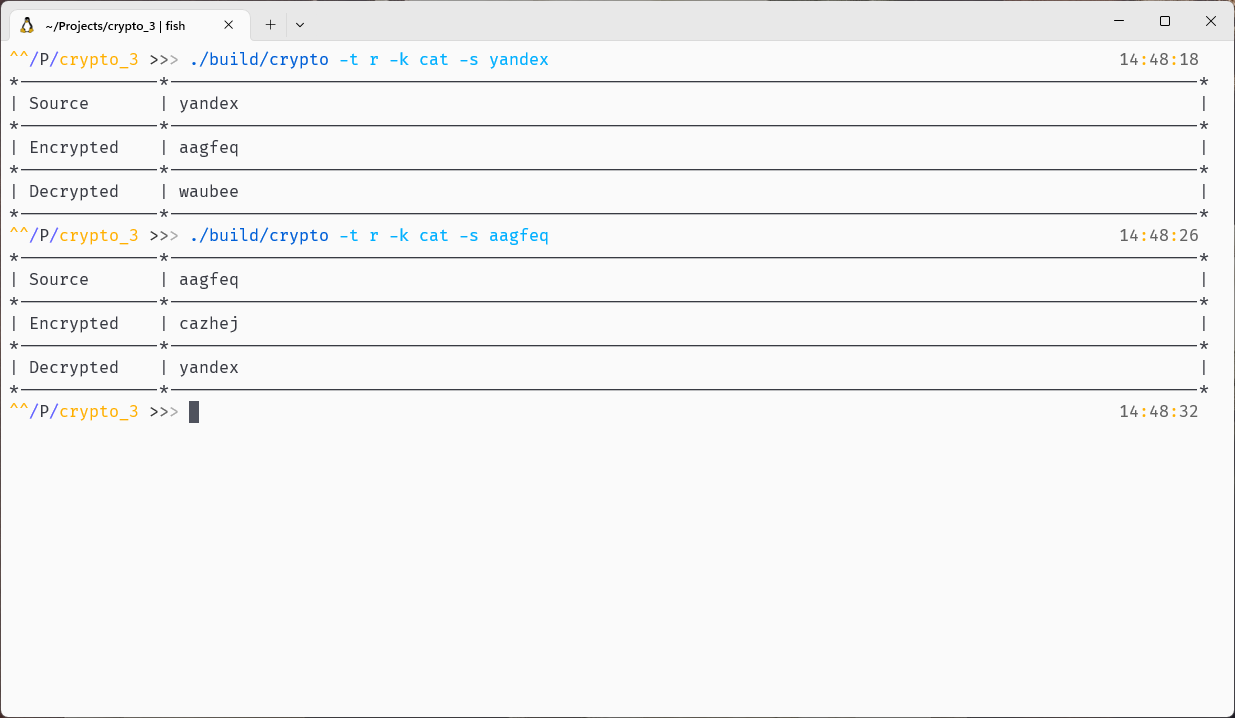
\includegraphics[width=0.9\textwidth]{03_00 (3)}
    \caption{Гамма - повторение короткого лозунга}
  \end{figure}

  \begin{figure}[H]
    \centering
    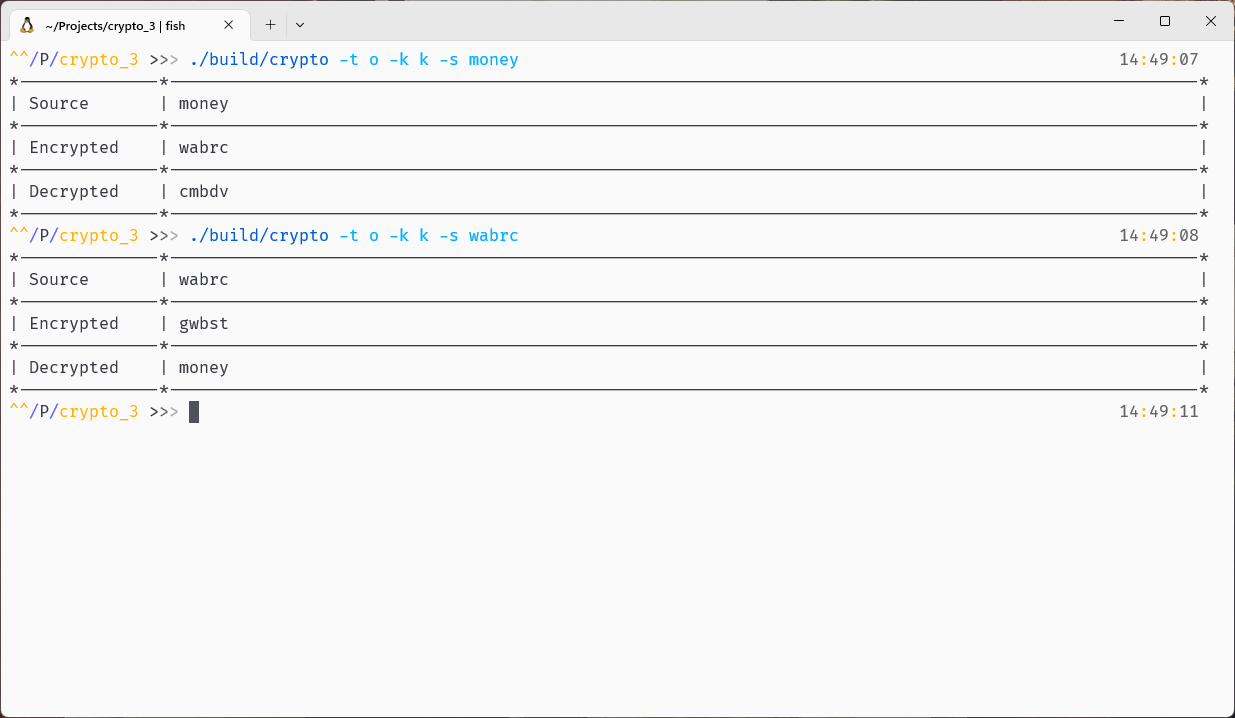
\includegraphics[width=0.9\textwidth]{03_00 (2)}
    \caption{Гамма - самогенерация по открытому тексту}
  \end{figure}

  \begin{figure}[H]
    \centering
    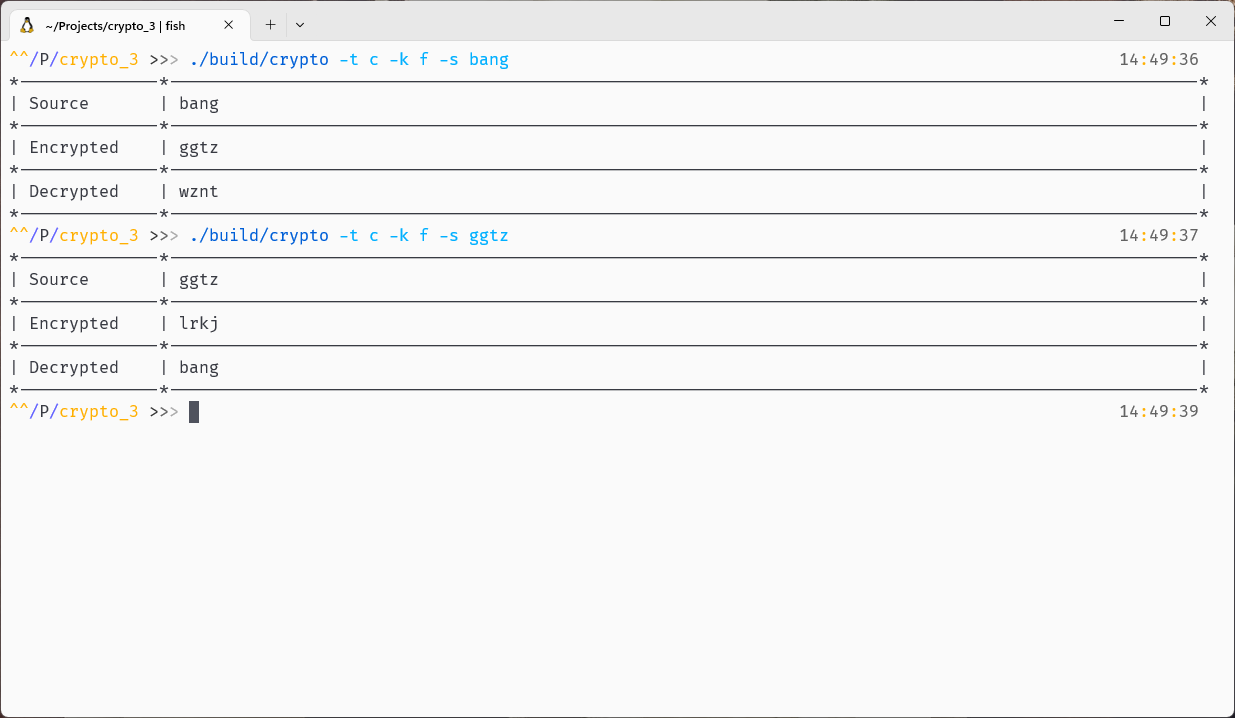
\includegraphics[width=0.9\textwidth]{03_00 (1)}
    \caption{Гамма - самогенерация по закрытому тексту}
  \end{figure}

  \newpage
  \section{Пример криптоанализа}

  Пусть есть некая последовательность-шифртекст:
  \begin{equation*}
    \begin{aligned}
      sxgeufrfcmtcrfoaegogvhjuwiqanktpfitcgsgejxeutaw\\
      glfftigwptlecnevhfuewgntgatgvftycqdzulpqkjpfpts\\
      poeujioispoephtigmxcnuvovuezqutqmfqfujenyaovtpi\\
      euwsffbzaovuongogvhfowbptuqacwsfaovuongogvhfowb\\
      ptuqbfcbvueeuwfgtetebosbtencdfqfujityhpcmjvoeks\\
      birfgiwgtscvfneevhfyosndbpdujetgvfpsfcsfxesabpf\\
      ytnopmiohosuongtiknhjomfypwrigaewplgeqaovthfcdv\\
      rmpxioqniqleaovthfcdvrmpxioqnlgeqaovthfcdvrmpxi\\
      oqniqleaovthfcdvrmpxioqnlgeqaovthfcdvrmpxioqniq\\
      leaovthfcdvrmpxioqnlgeqaovthfcdvrspoephtigmxcnu\\
      vovuezqutqmfqfujenyaovtpieuwsffbzaovuongogvhfow\\
      bptuqacwsfaovuongogvhfowbptuqbfcbvueeuwfgtetebo\\
      sbtencdfqfujityhpcmjvoeksbirfgiwgtscvfneevhfyos\\
      ndbpdujetgvfpsfcsfxesabpfytnopmiohosuongtiknhuw\\
      fgtetebosbtencdfqfujityhpcmjvoeksbirfgiwgtscvfn\\
      eevhfyosndbpdujetgvfpsfcsfxesabpfytnopmiohosuon\\
      gtiknhuwfgtetebosbtencdfqfujityhpcmjvoeksbirfgi\\
      wgtscvfneevhfyosndbpdujetgvfpsfcsfxesabpfytnopm\\
      iohosuongtiknhuwfgtetebosbtencdfqfujityhpcmjvoe\\
      ksbirfgiwgtscvfneevhfyosndbpdujetgvfpsfcsfxesab\\
      pfytnopmiohosuongtiknhuwfgtetebosbtencdfqfujity\\
      hpcmjvoeksbirfgiwgtscvfneevhfyosndbpdujetgvfpsf\\
      csfxesabpfytnopmiohosuongtiknhuwfgtetebosbtencd\\
      fqfujityhpcmjvoeksbirfgiwgtscvfneevhfyosndbpduj\\
      etgvfpsfcsfxesabpfytnopmiohosuongtiknh
    \end{aligned}
  \end{equation*}

  Начнем с поиска длины ключа, для этого определим количество повторяющихся
  символов для различных значений сдвига. Чаще всего встречалось количество повторений,
  равное 16, елси точнее, то для сдвигов:
  \begin{equation}
    \begin{aligned}
    \{&395, 491, 503, 563, 566, 596, 613, 632, 652, 659,\\
           &682, 685, 713, 746, 760, 769, 788, 793, 799, 820,\\
           &835, 838, 844, 846, 882, 927, 966, 981, 1053\}
    \end{aligned}  
  \end{equation}

  Наиболее часто-встречающаяся разница между соседними элементами этого списка равна 3,
  поэтому можем сделать вывод о том, что ключ с наибольшей вероятностью состоял из 3 символов.

  Теперь делим весь шифртекст на 3 группы, над каждой из которых проводим частотный анализ:

  \begin{figure}[H]
    \centering
    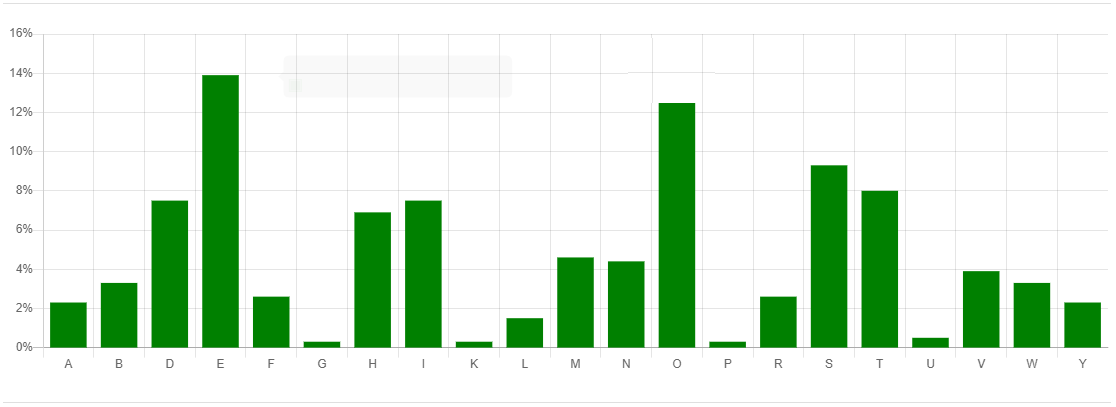
\includegraphics[width=\textwidth]{03_0004}
    \caption{Частотный анализ первой группы}
  \end{figure}

  \begin{figure}[H]
    \centering
    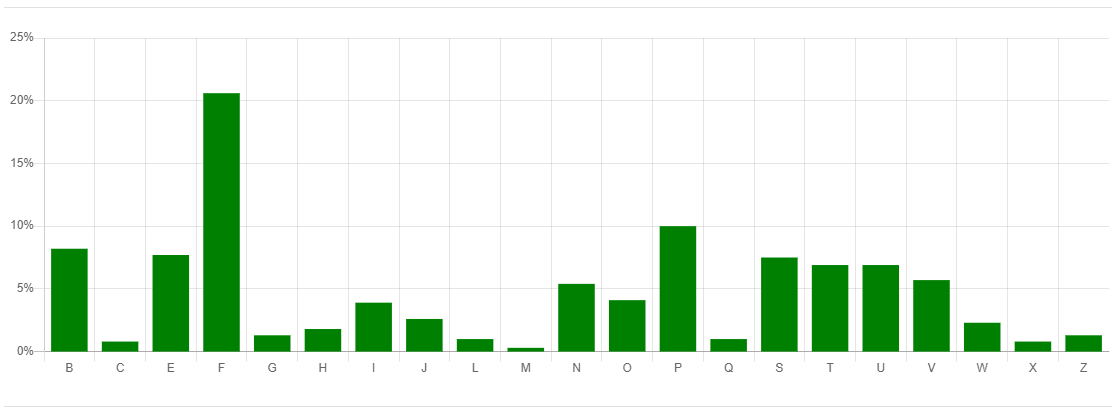
\includegraphics[width=\textwidth]{03_0005}
    \caption{Частотный анализ второй группы}
  \end{figure}

  \begin{figure}[H]
    \centering
    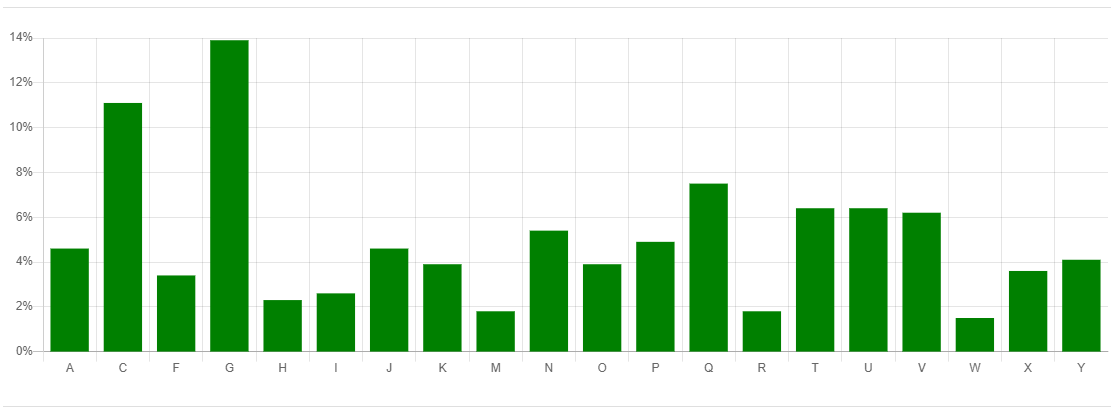
\includegraphics[width=\textwidth]{03_0006}
    \caption{Частотный анализ третьей группы}
  \end{figure}

  Попробуем составить ключ исходя из того, что наиболее частовстречающаяся буква английского алфавита - \textbf{E}.
  Рассмотрим расстояние от нее до наиболее часто встречающейся буквы каждой группы и будем
  использовать его как символ ключа.

  Для первой группы самый частый символ - \textbf{E}, его расстояние от \textbf{E} равно нулю,
  следовательно первый символ ключа - \textbf{A}.
  Для второй группы расстояние между \textbf{F} и \textbf{E} равно единице, поэтому второй символ ключа
  \textbf{B}. Для третьей же группы расстояние равно 2, поэтому последний символ ключа - \textbf{C}.

  Выполним расшифрование при помощи ключа \textbf{ABC}:
  \begin{equation}
    \begin{aligned}
      Sweet \text{ } dreams \text{ } are \text{ } made \text{ } of \text{ } this \\
      Who \text{ } am \text{ } I \text{ } to \text{ } disagree? \\
      I've \text{ } traveled \text{ } the \text{ } world \text{ } and \text{ } the \text{ } seven \text{ } seas \\
      Everybody's \text{ } lookin' \text{ } for \text{ } something \\
      \dots
    \end{aligned}
  \end{equation}

  Похоже на настоящий открытый текст.

  \newpage
  \section{Вывод}

  В ходе данной работы мне удалось программно реализовать за- и расшифрование текстов
  с помощью шифра Виженера с различными методами выработки гаммы, а также провести его криптоанализ.

  Наиболее устойчив к взлому шифр Виженера, использующий генериацию гаммы повторением короткого лозунга,
  так как такую модификацию сложнее всего сломать подбором. Однако шифр все же поддается
  частотному анализу, что не делает его полностью безопасным.

  Другие модификации легко взламываются с помощью полного перебора, так как там требуется перебрать
  совсем небольшое множество различных ключей.

\end{document}
